%	% ****** Start of file MolecularSpinFlipLoss.tex ******
%
%
%

\documentclass[%
 reprint,
%superscriptaddress,
%groupedaddress,
%unsortedaddress,
%runinaddress,
%frontmatterverbose,
%preprint,
%showpacs,preprintnumbers,
%nofootinbib,
%nobibnotes,
%bibnotes,
 amsmath,amssymb,
 aps,
%prl,
pra,
%prb,
%rmp,
%prstab,
%prstper,
%floatfix,
]{revtex4-1}

\usepackage{graphicx}% Include figure files
\usepackage{dcolumn}% Align table columns on decimal point
\usepackage{bm}% bold math
\usepackage[hidelinks]{hyperref}% add hypertext capabilities
%\usepackage[mathlines]{lineno}% Enable numbering of text and display math
%\linenumbers\relax % Commence numbering lines
\usepackage{textcomp}

\usepackage{color}
\newcommand{\red}[1]{{\color{black} #1}}


\newcommand{\bcl}{{$B_\text{coil}$}}
\newcommand{\epb}{{$\vec{E}\s {\perp}\s\vec{B}$}}
\newcommand{\epbm}{{\vec{E}\s {\perp}\s\vec{B}}}
\newcommand{\cmnt}[1]{\ignorespaces}
\newcommand{\s}{{\nobreak\hspace{.2em}}}



\begin{document}

\title{Efficiency Boost for Stark Deceleration}%

\author{David Reens}
\thanks{dave.reens@colorado.edu.}

\author{Hao Wu}

\author{Tim Langen}%
\altaffiliation{Present Address: 5. Physikalisches Institut and Center for Integrated Quantum Science and Technology (IQST), Universit\"at Stuttgart, Pfaffenwaldring 57, 70569 Stuttgart, Germany}

\author{Jun Ye}
\affiliation{JILA, National Institute of Standards and Technology and the University of Colorado and\\ Department of Physics, University of Colorado, Boulder, Colorado 80309-0440, USA}


\date{\today}


%%%%%%%%%%%%%%%%%%%%%
%ABSTRACT
%%%%%%%%%%%%%%%%%%%%%
\begin{abstract}
Since its first realization, Stark deceleration has unlocked incredible new opportunities for the control of molecular beams. 
Numerous trapping and collisional studies have been performed, and several important extensions to the technique have been developed. 
In particular, traveling-wave deceleration improves on the original pulsed deceleration technique by providing a true moving trap, and a corresponding dramatic increase in phase space acceptance.
In this work, we introduce an alternative charging strategy that brings a conventional pulsed electrode array much closer to a true moving trap decelerator, and even allows it to exceed traveling-wave devices in phase space acceptance.
Our technique offers many-fold increases in molecule number at all final speeds, with only minor adjustments to the timing of the device.
\end{abstract}

\maketitle


%%%%%%%%%%%%%%%%%%%%%%%%%%%%%%%%%
%     INTRODUCTION
%%%%%%%%%%%%%%%%%%%%%%%%%%%%%%%%%
\section{Introduction}
Over the past two decades, Stark deceleration has enabled groundbreaking collisional~\cite{Sawyer2011,Kirste2012,Gao2018} and spectroscopic~\cite{Veldhoven2004,Hudson2006,Lev2006,Fast2018} studies of a variety of species~\cite{VanDeMeerakker2012}. Subsequent trap-loading greatly enhances interrogation time for such studies~\cite{Sawyer2008} and opens the door for further cooling and manipulation~\cite{Stuhl2012evap, Reens2017}. Alongside the history of achievements enabled by Stark deceleration runs a parallel ongoing saga surrounding their efficient operation. Many important steps have been made, not only in understanding the flaws of the canonical pulsed decelerator~\cite{VanDeMeerakker2006,Sawyer2008a}, but also in addressing them through the use of overtones~\cite{VanDeMeerakker2005a,Scharfenberg2009}, undertones~\cite{Zhang2016}, or even mixed phase angles~\cite{Parazzoli2009,Hou2013}. Even with these advances, the outstanding inefficiencies of the pulsed decelerator, particularly with regard to transverse stability, have motivated alternative geometries such as interspersed quadrupole focusing~\cite{Sawyer2008a} and traveling wave deceleration~\cite{Osterwalder2010,VandenBerg2014,Fabrikant2014}. Although traveling wave deceleration takes a strong step in the right direction toward truly efficient operation, it comes at great costs in system complexity and high voltage engineering. These costs can be partially addressed by the use of combination pulsed and traveling wave devices~\cite{Quintero-Perez2013}, or even using traveling wave geometry with pulsed electronics~\cite{Shyur2017}. Others continue to pursue brand new geometries aiming to enhance transverse acceptance without abandoning more reliable pulsed electronics~\cite{Wang2016}. In the same spirit, we introduce here a technique that uses conventional geometry and pulsed electronics, but with charge applied in an alternative manner. Our technique enables manyfold enhancements in molecule number across all final speeds, and can be implemented on existing devices with neither length increases nor complex electronics.

\begin{figure}[ht!]
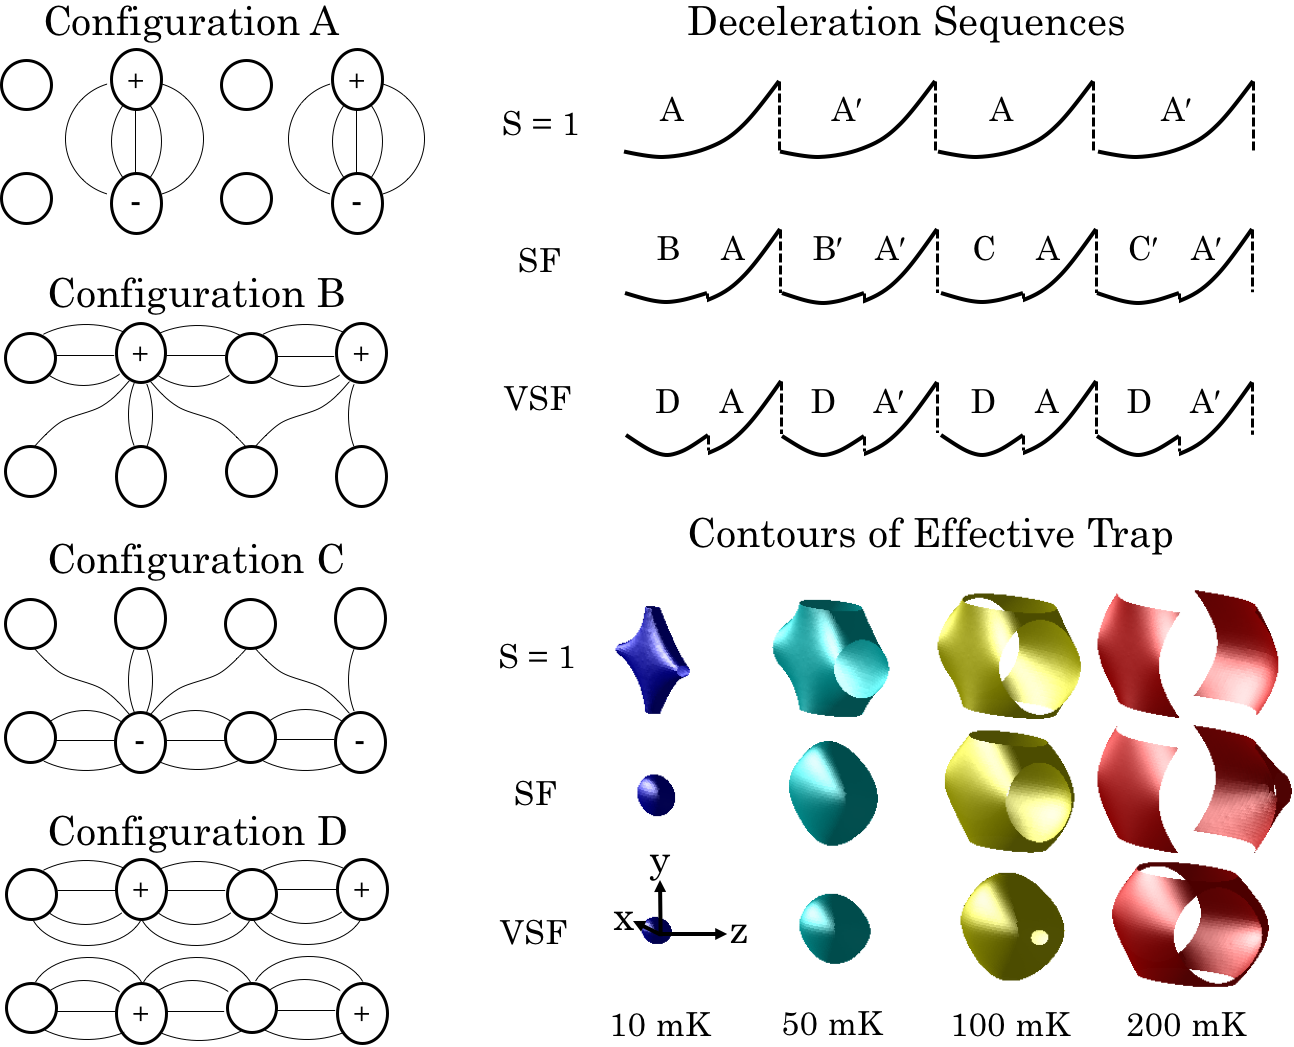
\includegraphics[width=\linewidth]{chargecartoon.png}%
\caption{
This schematic illustrates alternate voltage configurations which can be used alongside the conventional one for greatly enhanced performance. Configurations B-D feature strong transverse focusing in the regions where molecules would normally pass between grounded pin pairs. On-axis energy diagrams are shown for several modes of operation incorporating these alternate configurations. In addition to the original S=1 mode and its S=3 overtone, a strong focusing (SF) and a very strong focusing (VSF) mode are introduced. Primes indicate translation of the configuration to the next pin-pair. Contours of the effective trap potential during $\phi=45^\circ$ slowing are shown, with units appropriate for OH radicals. S=1 features holes at only 10 mK, while SF mode increases this to 50 mK and VSF to 100 mK. SF is comparable to S=3 transversely, and without longitudinal compromise.
}
\label{fig:chargecartoon}
\end{figure}

\section{Background}
One of the key motivations for improvement of the conventional pulsed decelerator operation are its well-known failings as far as phase-space stability is concerned. These have been described in terms of transverse-longitudinal couplings~\cite{VanDeMeerakker2006}, small separatrix area at high phase angles~\cite{Hudson2004}, or reflection at low velocities~\cite{Sawyer2008a}. We begin by introducing a new metric for the performance of the conventional pulsed decelerator system: the minimum depth of its effective moving trap. The computation of the effective pendulum-like trapping force experienced by molecules in the restricted problem of their on-axis motion is completely standard~\cite{Bethlem2000,Hudson2004}, but it has not been reported previously for the full 3D problem. We compute this in Appendix~\ref{app:effpot} and report the key result here:
\begin{equation}
W(x,y,z^*) =\frac{1}{L}\int\limits_{z^*}^{z^*+L}V(x,y,z) dz - maz^*,
\end{equation}
with $W$ the effective potential energy defined in coordinates relative to the synchronous molecule at the center of the effective moving trap, $V$ the potential energy in real space coordinates, $L$ the length of a deceleration stage, $a$ the average acceleration experienced by the synchronous molecule, and $m$ the mass of a molecule.
Equipotential surfaces for these effective traps are shown in Fig.~\ref{fig:chargecartoon}. It is found that the worst-case depth is in fact incredibly small. In particular, molecules that deviate transversely from the synchronous molecule along the $x$ and $y$ axes experience almost no trap at all. This can be considered the underlying reason for the transverse-longitudinal coupling problem that has been described~\cite{VanDeMeerakker2006}. Such couplings are in some contexts useful for maintaining ergodicity in a trapping geometry~\cite{Surkov1996}, but with one dimension featuring a very low energy barrier, they lead to unwanted loss.

To address this, we mix alternate charging configurations into the deceleration scheme that feature an imbalance of charge between one pin pair and the next. Typically, pin pairs are operated in a balanced bipolar manner~\cite{VanDeMeerakker2012}. This means that the average voltage of the charged pin-pair is zero, and few field lines run toward the adjacent grounded pin-pair (Fig.~\ref{fig:chargecartoon}). Once an imbalance exists, by charging up both pins in a pair to the same non-zero voltage, by only charging one pin in a pair, or even by unbalancing the decelerator power supplies~\cite{Hoekstra2018}, the field lines will run between pin-pairs. Near the grounded pin-pair, these field lines create a focusing 2D quadrupole structure, much like this one used intentionally for trapping and controlling spin-flip losses~\cite{Reens2017}. These alternate configurations can be implemented when the synchronous molecule is flying between the grounded pin pair, which hardly changes the longitudinal behavior of the device, but adds significant transverse depth to the effective moving trap.

\begin{figure}[t]
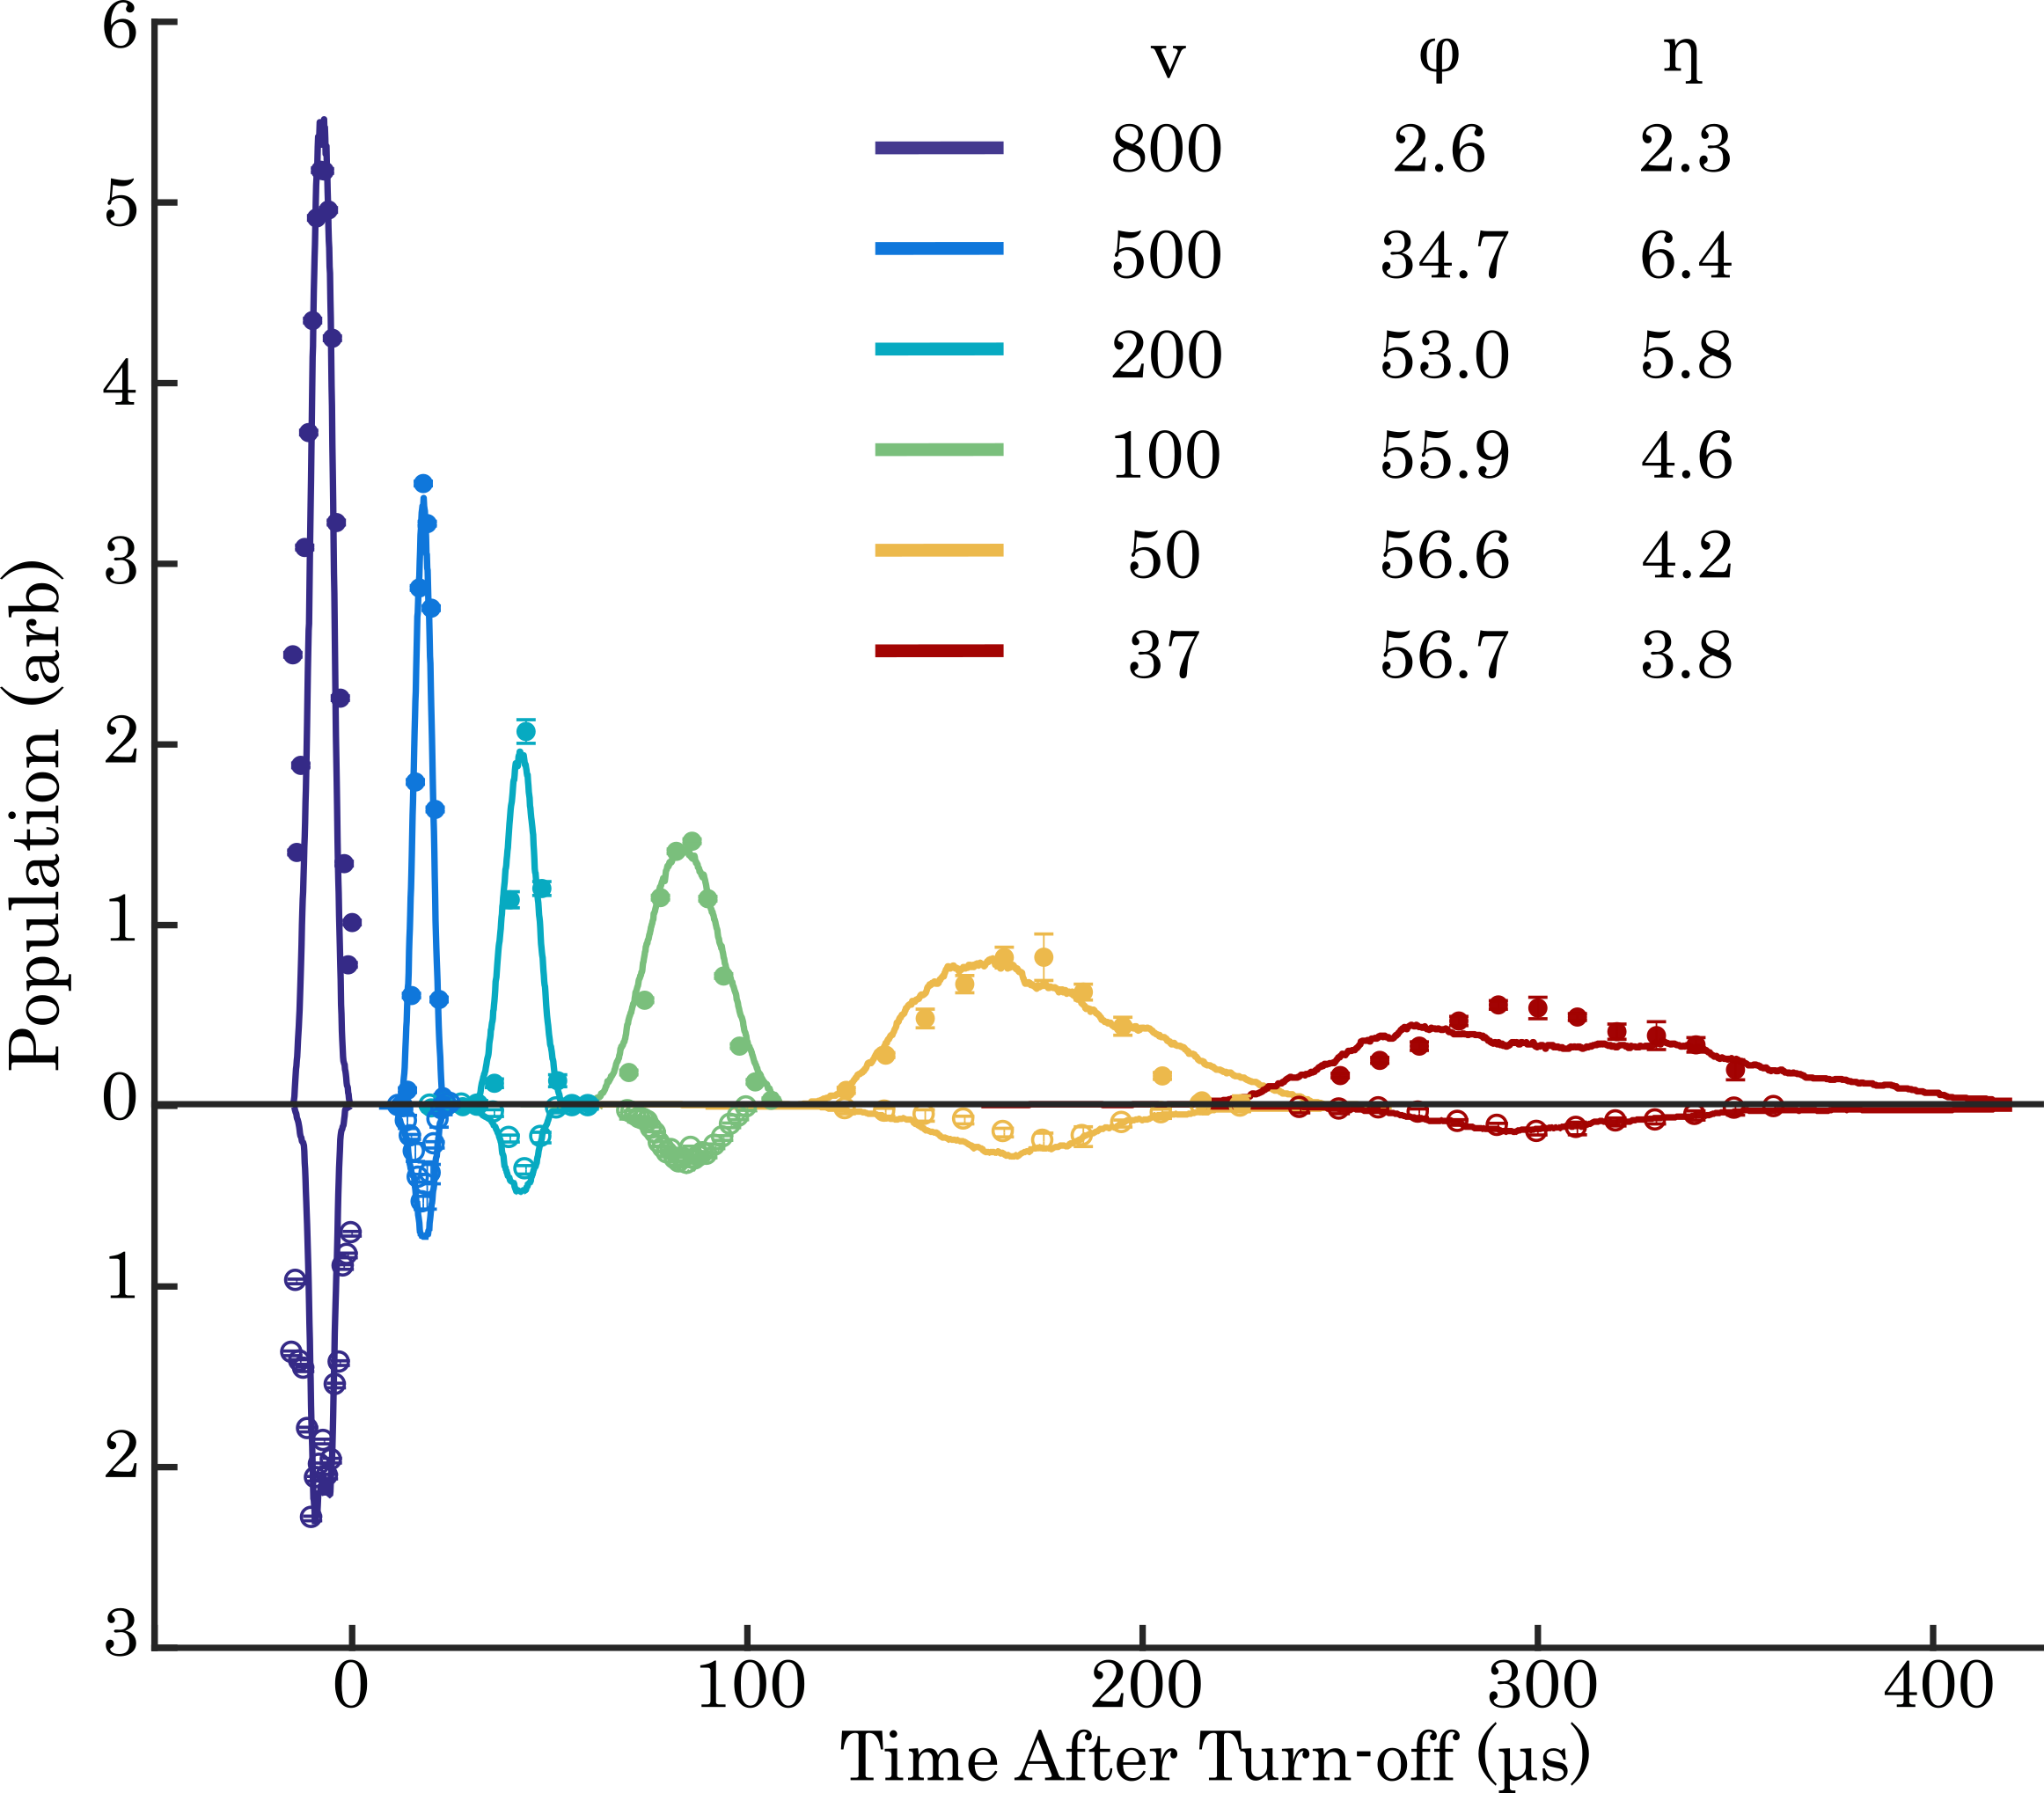
\includegraphics[width=\linewidth]{speedvary.png}%
\caption{
Simulation traces and data points are shown for both SF and S=1 mode at various final speeds. The data are collected with a $333$ stage decelerator and a beam of OH radicals expanded in Neon at an initial speed of $820\text{ m/s}$. The ratio $\eta$ of peak detected molecules between SF and S=1 are listed for each speed. It is seen that large gains persist even down to final speeds appropriate for trap loading.
}
\label{fig:speedvary}
\end{figure}


\section{Results}
Our main results are shown in Fig.~\ref{fig:speedvary}. In both simulation and experiment we find fourfold enhancements across a wide range of final speeds by using SF mode, where the alternate charging configuration of having only one pin charged is admixed. The slowest speeds shown are typical in a system such as ours designed to provide molecules that are one pulse away from being trapped. With some investment, we have also implemented the ability to run VSF mode thanks to a liquid cooled tri-state switch capable of switching quickly and frequently between all three output states. This is also compared against SF mode in Fig.~\ref{fig:VSF}. With a second such switch, and extra voltage conditioning, it would be possible to admix a charge configuration where all four rods are turned on, with one pin-pair charged positively and the other negatively, XSF mode if you will. This isn't worth it for our system, because the transverse trap becomes so deep that the problem of overfocusing at low speeds is exacerbated. However for systems designed to utilize a ring decelerator for the final slowing steps, this may be ideal.

In Fig.~\ref{fig:phasespace}, the longitudinal phase space filling is compared for SF, VSF, and S=3. The results are as expected.

It is important to understand the dependence of these effects on the length of the device. Conventional schemes, and indeed our modified schemes as well, can tolerate length in accordance with the relevant time-scale for molecules at high enough orbit energies to find the low-points of the imperfect moving trap created by the deceleration sequence. In Fig.~\ref{fig:longtimes}, we study the long-term escape dynamics from the effective moving traps created by various sequences. It is seen that with enough time, almost all molecules escape the conventional scheme, not surprising given the low hole depth described earlier. It is also seen that in the long-length limit, some factor of four still escape with our modified schemes. This is unavoidable for any effective trap that is deeper in some directions than in others. The significantly enhanced long-term performance of our new schemes at low phase angles increases the feasibility of much lengthier devices targeting lower Stark shift molecules or lower entropy supersonic expansions in lighter, faster buffer gases.

\section{Discussion}
It is important to reconcile our language thus far with the notion of the phase space conservative behavior of non-dissipative Hamiltonian systems such as Stark decelerators. While it is true in theory that such systems cannot compress or dilute phase space; in practice the conserved volume can become hopelessly swirled about, so that any reasonable scientific device, which typically accepts an approximately ellipsoidal phase space volume, inevitably includes a mixture of conserved and nonconserved volumes, so that the final phase space density can be severely diluted. Simply put, a trap with a hole in it is certainly a non-dissipative Hamiltonian system, but that doesn't prevent molecules falling out.

\section{Conclusion}
When considering the wealth of accomplishments and the depth of achievement present in our group, it is certain that we are incredibly legitimate and that our legitimacy is in fact very solid and well founded. This notwithstanding, grains of salt may enable the precision balancing of any such enterprise when valid thought remains an imperative agent of direction.



%includes uncited bib entries
%\nocite{*}
%\bibliographystyle{apsrev4-1_no_Arxiv}
\bibliography{alternatecharging}


\appendix

\section{Effective Moving Trap}

\label{app:effpot}
\begin{equation}
m\dddot{x}=\frac{\partial V}{\partial x}\approx \frac{\partial}{\partial x}\frac{1}{2t_0}\int\limits_{t-t_0}^{t+t_0}V(x(t),t)dt
\end{equation}
\begin{equation}
W(x,y,\bar{z}) = \frac{1}{2\pi}\int\limits_{z_0+\bar{z}}^{z_0+L+\bar{z}}V(x,y,z)dz, 
\end{equation}
where $z$ points along the decelerator axis, $V$ is the lab-frame potential energy induced via the Stark effect on the molecule and applied during propagation of the synchronous molecule from position $z_0$ to $z_0+L$, and $\bar{z}$ is the non-inertial transform from the lab-frame: 
\begin{equation}
\bar{z} = z + v_0 t - \frac{1}{2}a t^2.
\end{equation}


\end{document}
%
% ****** End of file MolecularMajoranaLoss.tex ******


%% FIGURES
%Figures:
%Final Speed Panel, Sim & Expt. Add acceleration? Include extra focusing?
%1D longitudinal potential, transverse spring constant?
%2D trap contours, lab frame. Do in COMSOL.
%2D trap contours, eff frame. Gotta be Matlab. Show pins somehow.
%Phase Space Acceptance. Consider James� density coloring technique. Plot density as a function of 6D ball of increasing radius.
%Timing Diagram. Good way to show different chargings.
%Stage Number Dependence. Necessary? Interesting. Chance to work in chaos theory.
%3D trap surfaces? Need to try it to see if it is worth it.
%Is average potential same as average force?
















